\RequirePackage[l2tabu, orthodox]{nag}

\documentclass[10pt]{scrartcl}
\usepackage[T1]{fontenc}
\usepackage{amsmath,amsfonts,amssymb}
\usepackage{mathtools}
\usepackage{cancel}
\usepackage{color,soul}
\usepackage[margin=2cm]{geometry}
\usepackage{enumerate}
\usepackage{graphicx}
\usepackage[colorlinks=true,urlcolor=blue]{hyperref}
\usepackage{floatrow}
\usepackage{deluxetable}
\usepackage{verbatim}
\usepackage{fancyvrb}
\usepackage{listings}
\usepackage{calc}
\usepackage{xfrac}
\usepackage{cleveref}
\usepackage[font=small]{caption}
\usepackage[font=scriptsize]{subcaption}
\usepackage[activate={true,nocompatibility},final,tracking=true,kerning=true,spacing=true,factor=1100,stretch=10,shrink=10]{microtype}
\SetTracking{encoding={*}, shape=sc}{40}

\microtypecontext{spacing=nonfrench}

\floatsetup{ 
  heightadjust=object,
  valign=t
}

\definecolor{Light}{gray}{.90}
\sethlcolor{Light}

\lstset{%
language=IDL,                   % choose the language of the code
basicstyle=\footnotesize\sffamily,%\ttfamily\footnotesize,       % the size of the fonts that are used for the code
numbers=left,                   % where to put the line-numbers
numberstyle=\footnotesize,      % the size of the fonts that are used for the line-numbers
stepnumber=1,                   % the step between two line-numbers. If it is 1 each line will be numbered
numbersep=5pt,                  % how far the line-numbers are from the code
showspaces=false,               % show spaces adding particular underscores
showstringspaces=false,         % underline spaces within strings
showtabs=false,                 % show tabs within strings adding particular underscores
frame=single,                   % adds a frame around the code
backgroundcolor=\color{Light},
columns=flexible,
tabsize=2,                      % sets default tabsize to 2 spaces
captionpos=b,                   % sets the caption-position to bottom
breaklines=true,                % sets automatic line breaking
breakatwhitespace=false,        % sets if automatic breaks should only happen at whitespace
escapeinside={\%*}{*)}          % if you want to add a comment within your code
}

\title{Why We Do What We Do (WWDWWD)}
\author{Jeren Suzuki}
\date{Last Edited \today}

\begin{document}

\maketitle
\pagenumbering{Roman}
\tableofcontents
\addcontentsline{toc}{section}{Introduction}
\clearpage
\pagenumbering{arabic}

\section*{Introduction} % (fold)
\label{sec:introduction}
\indent This document is an attempt to organize the decision behind our methods in the grand scheme plan of extracting useful data from our image. I will try to organize it in parts so that it will be easier to follow.
% section introduction (end)

\section{Data Acquisition} % (fold)
\label{sec:data_acquisition}
Even before we have an image, we have to talk to the camera, so to speak. This involves installing the PvPAPI SDK on an ubuntu machine connecting the machine directly to the camera through an ethernet port, then manually setting the network interface to lie on the same subnet as the camera (the camera can't change IP so it must be done on the computer). Once the IP and subnet mask (and gateway too?) are configured correctly, the camera can be set to take pictures by navigating to the \texttt{AVT GiGE SDK} $\rightarrow$ \texttt{bin-pc} $\rightarrow$ \texttt{x64} directory and running \texttt{SampleViewer}. You should see a widget appear with the camera listed in the interface. Setting up the camera is beyond the scope of this document but I have partial instructions in \texttt{sdkrefman} and Nicole has printed out instructions in one of her binders. 

\subsection{Setting up image} % (fold)
\label{sub:setting_up_image}

Now that we've setup the camera, we need something to take pictures of. We simulate a solar image based on the images we received from Albert. To do this, we need:

\begin{itemize}
    \item Pixel pitch of camera sensor (physical size of pixel)\\   
        If you don't have the pixel pitch, use the sensor dimensions against the image resolution
    \item Image resolution (4192x3264, etc)
    \item Distance from focal plane to imaged plane
    \item Focal length of lens
\end{itemize}

we stick them into this equation:

\begin{equation}
    \frac{\textrm{pixel pitch}}{\textrm{focal length}} = \frac{\textrm{physical length of a pixel in the image}}{\textrm{distance from camera to sheet of paper}-\textrm{focal length}}
\end{equation}

If we want the sun to be $N$ pixels wide (corresponding to $M$ cm), then open an image editor at 300 pixels/cm and make a sun 

\begin{align}
    300 ~\frac{\textrm{pixels}}{\textrm{cm}} \cdot M ~\textrm{cm}\\
    300 ~\frac{\textrm{pixels}}{\cancel{\textrm{cm}}} \cdot M ~\cancel{\textrm{cm}}\\
    300 \cdot M~\textrm{pixels wide}
\end{align}

\Cref{ohyeah} compares the \emph{fiducials} we were testing to the starting image we based them off. \emph{Fiducials}. Not the shape/size of the sun.

\begin{figure}[!ht]
    \ffigbox[][\FBheight]{%
    \begin{subfloatrow}[2]%
        \ffigbox[\FBwidth]%
       {%
       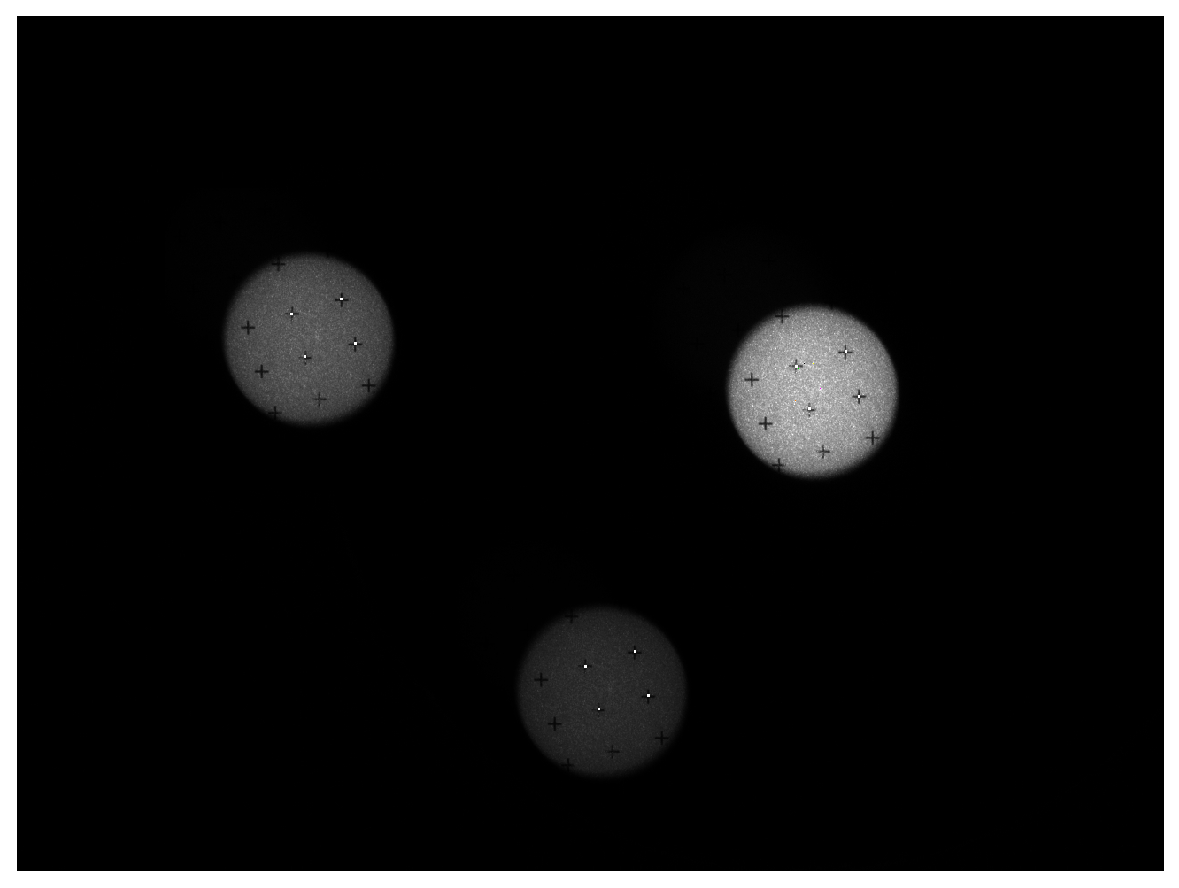
\includegraphics[width=.5\textwidth]{../plots_tables_images/best4_actual.eps}%
       }%
       {%
       \caption{The image we based the fiducial dimensions on (and only fiducial dimensions, not solar dimensions)}%
       }%
        \ffigbox[\Xhsize]%
       {%
       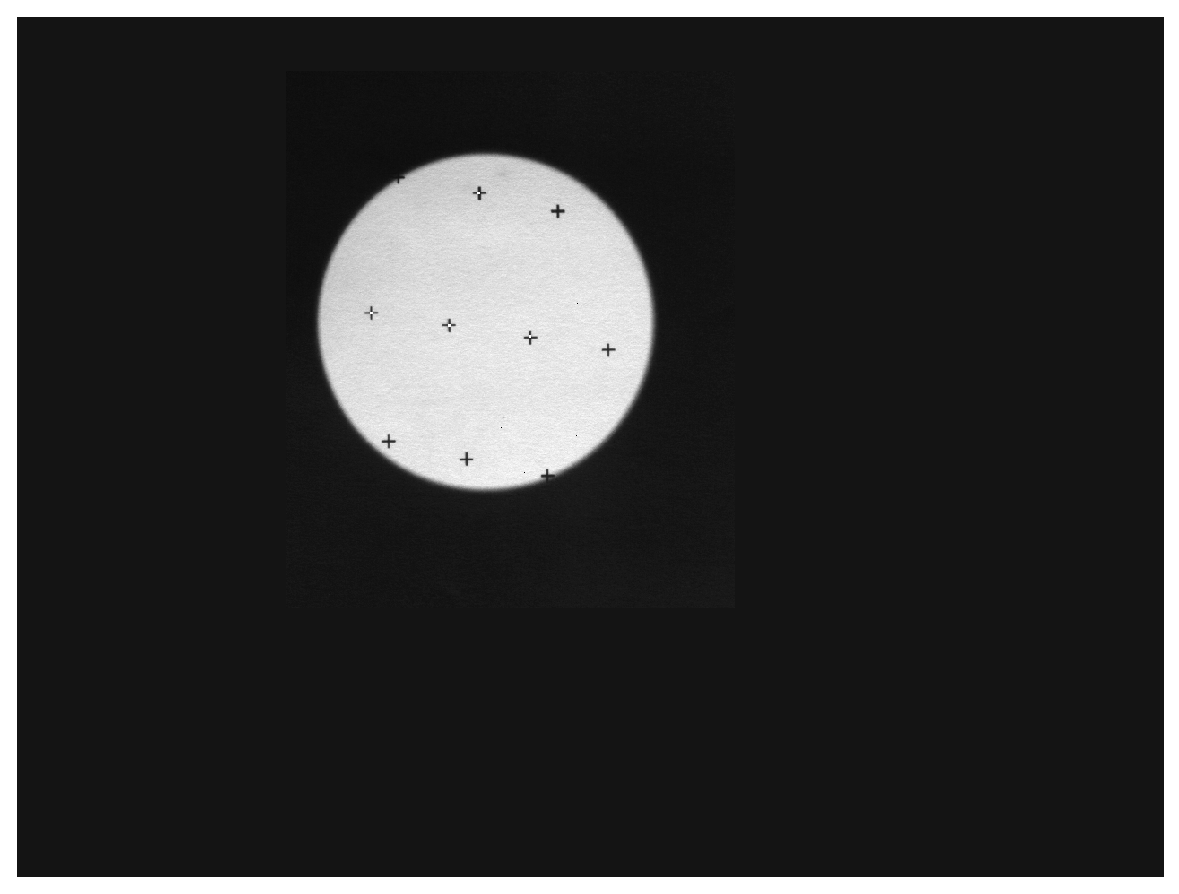
\includegraphics[width=.5\textwidth]{../plots_tables_images/best4.eps}%
       }%
       {%
       \caption{Our simulated image. Ignore the hilariously large sun and notice the fiducials are about the same size.}%
       }%
    \end{subfloatrow}}{\caption{}\label{ohyeah}}%
\end{figure}

% subsection setting_up_image (end)
% section data_acquisition (end)

\section{Handling 2D Image} % (fold)
\label{sec:handling_2d_image}

\subsection{File Formats} % (fold)
\label{sub:file_formats}
In an effort to maintain maximum portability across all platforms, we saved all our images in the \emph{FITS} file format. Any images received for testing purposes (for example, the ones from Albert), I opened in IDL and converted into FITS. 

\subsubsection{Specific to Photos from a DLSR} % (fold)
 \label{ssub:specific_to_photos_from_a_dlsr}
When dealing with images generated with my DLSR when taking bundle mask images, they had to be converted from RAW into 16 bit TIFF then loaded into IDL. JPEG files introduced artifacts and the actual range of a pixel in a JPEG file wasn't as high. TIFF files were considered filled with unsigned integers while JPEG files only ranged in BYTE values. If there is the option, use TIFF files. The only problem is that TIFF files are incredibly large.  

Also, photos taken from my camera come with three channels, red, green, and blue. When doing image analysis, I chose the image with the most contrast when on a black-white color table. If my memory serves me right, the fits files contain the first channel of the 3 channel image when loaded with either \hl{\texttt{READ\_JPEG}} or \hl{\texttt{READ\_TIFF}}, corresponding to the red channel.
% subsubsection specific_to_photos_from_a_dlsr (end) 

% subsection file_formats (end)

% section handling_2d_image (end)

\section{Skimming the Top Off} % (fold)
\label{sec:skimming_the_top_off}
We want to eliminate any outlier pixels that are way too bright so we sort our 2D image as a 1D array and mask out the top 1\% (or .1\%, whatever) of the pixels for our threshold. Even though in the sample images provided by Albert there are no bright outlier pixels, eliminating the brightest pixels poses no detrimental affect to image processing.
% section skimming_the_top_off (end)

\section{Deciding Whether or Not to Use Image} % (fold)
\label{sec:deciding_whether_or_not_to_use_image}
% Include all the checks we do

Technically, this is more whether or not to \emph{keep} the image


To make sure that we identify the appropriate centers of the sun, we make sure that we know how many are actually in the picture. First, we check if there are any pixels on the border of the image that are a significantly higher value than the mode of the image. If we see X pixels on the border, then one of the suns is cut off. If we see X and Y pixels on the border, then we take into account 2 cut-off suns. We must make sure that if we see no sun-pxiels on theborder that there isn't a chance that we missed a sun altogether and there are only 2 suns in the image. Still need to work on this.

After the centers of every solar-shaped object is found, two checks are made:

\begin{enumerate}
    \item Is the center too close to the edge?
    \item Is the center too close to certain edges after being rotated 45$^\circ$?
\end{enumerate}

Previous methods included:

\begin{enumerate}
    \item Check for bright pixels on image border, if number of continuous bright pixels exceeds a threshold, the general area is considered ``\emph{bad}''
    \item Count bright pixels on image border mask, if number exceeds a certain threshold, use further processing to determine where in the image the bad sun lies
\end{enumerate}

We chose the rotation method because it quickly and efficiently deals with the problem that the bottom corners will never see any data. The problem with using a border mask was that it's easy to construct for a rectangle, but when you start throwing in angles, the amount of time it takes to construct the mask increases quickly. To deal with the bottom two corners, one method was to make triangle matrices with 0s and 1s and then append them to the bottom corners of a large rectangular matrix. Another method was to use \hl{\texttt{shift}} to move around the rectangular matrix within a larger matrix, multiply the shifted matrices together, and then crop the final matrix down to the original size. 

Still within the realm of rotating the image, the first attempt involved rotating the entire image and then checking the distance from the edge. This was completely unnecessary since at this point we already have the center positions of the solar shaped objects and thus only need to apply a rotation function onto a single ($x,y$) coordinate. 

\begin{figure}[!ht]
    \ffigbox[][\FBheight]{%
    \begin{subfloatrow}[2]%
        \ffigbox[\FBwidth]%
       {%
       
\includegraphics[width=.5\textwidth]{../plots_tables_images/cutcorner.eps}%
       }%
       {%
       \caption{The image mask with the bottom corners as no-data zones}%
       }%
        \ffigbox[\Xhsize]%
       {%
       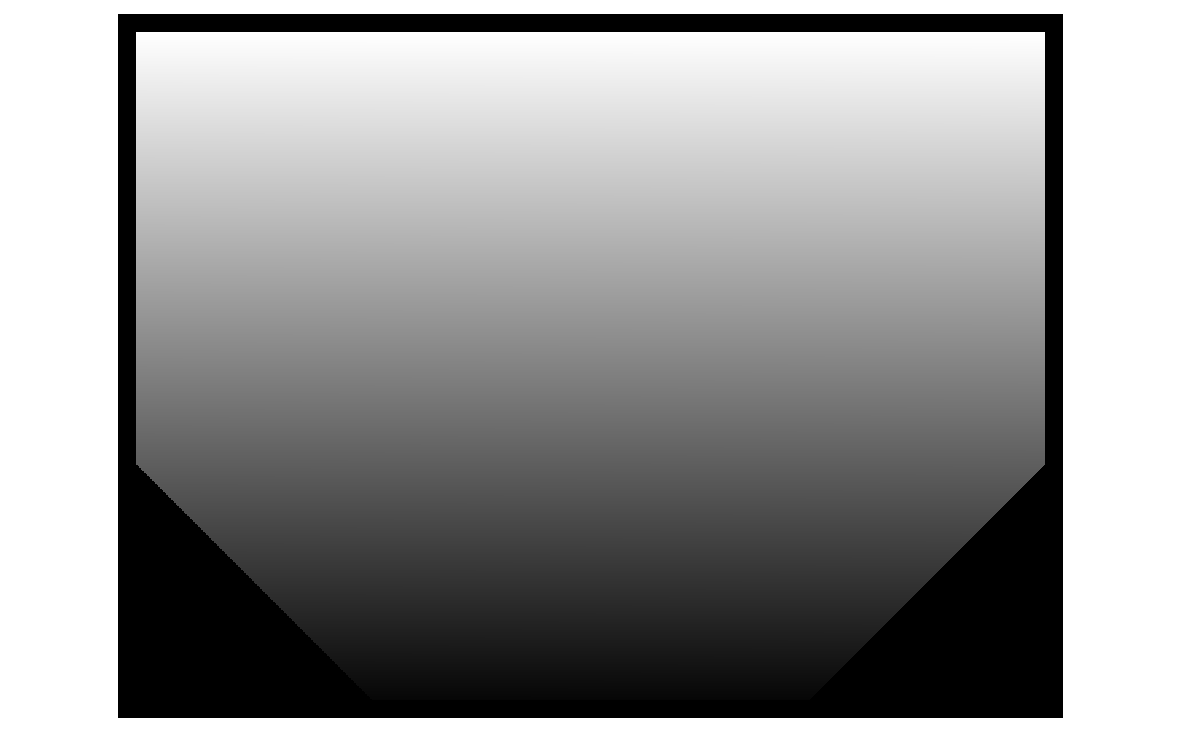
\includegraphics[width=.5\textwidth]{../plots_tables_images/cutcornerwborder.eps}%
       }%
       {%
       \caption{What the initial attempts at border-masking achieved, although at the heavy cost of time. If there were any solar pixels identified in that border region, then further processing would occur.}%
       }%
    \end{subfloatrow}}{\caption{}\label{corner}}%
\end{figure}

\begin{figure}[!ht]
    \ffigbox[][\FBheight]{%
    \begin{subfloatrow}[2]%
        \ffigbox[\FBwidth]%
       {%
       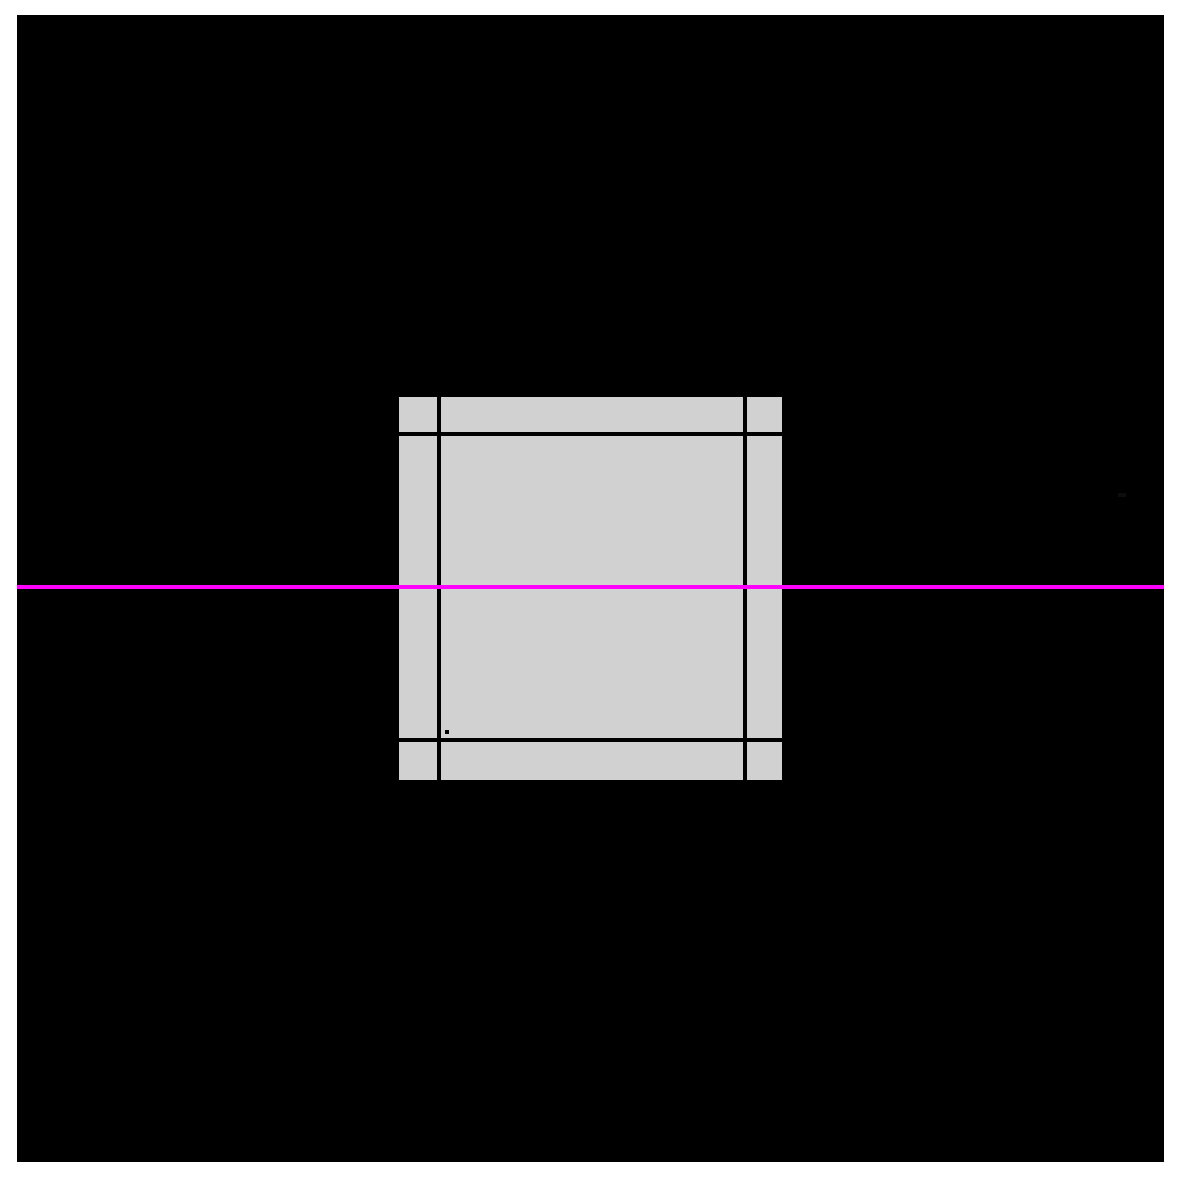
\includegraphics[width=.5\textwidth]{../plots_tables_images/firstcheck.eps}%
       }%
       {%
       \caption{The gray square simulates the solar image with 3 suns. The black dot is the center of a sun that would otherwise be considered ``good'' by the program since it doesn't take into account the bottom corners.}%
       }%
        \ffigbox[\Xhsize]%
       {%
       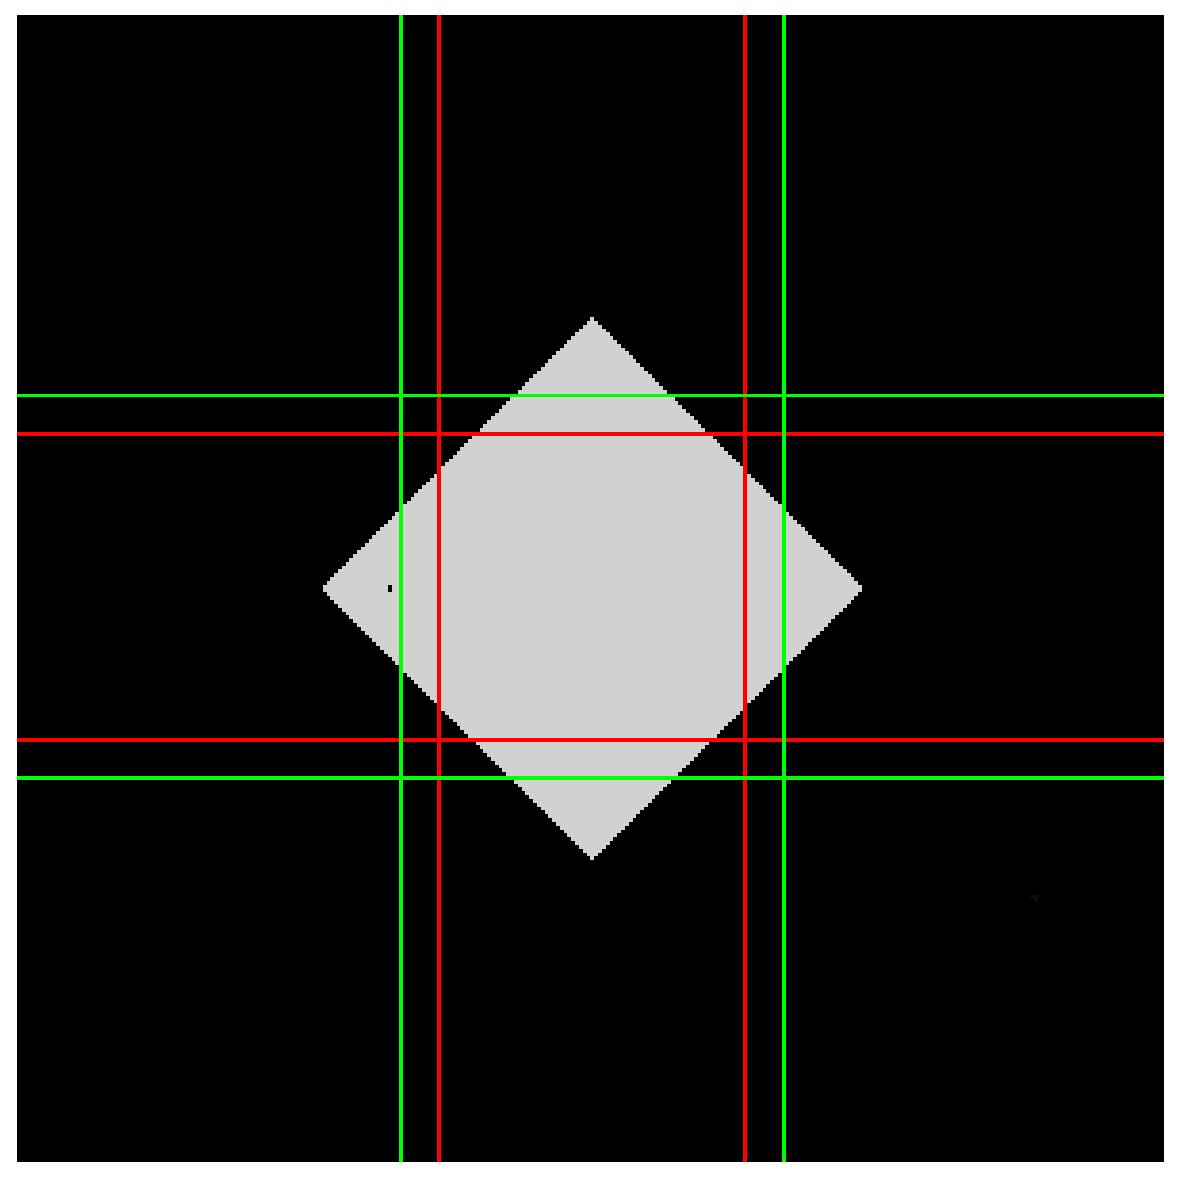
\includegraphics[width=.5\textwidth]{../plots_tables_images/seccheck.eps}%
       }%
       {%
       \caption{With the image rotated 45$^\circ$ (but in reality, only the black dot is rotated. the entire array is rotated here to show the effect), the black dot now lies beyond the green line, which is the original border of the gray square. The left vertical and bottom horizontal green line mark the boundary regions for the bottom two corners. This method is fast.}%
       }%
    \end{subfloatrow}}{\caption{}\label{cchecks}}%
\end{figure}

% section deciding_whether_or_not_to_use_image (end)

\section{Finding Centers of Sun(s)} % (fold)
\label{sec:finding_centers_of_sun}

We used a mask centroiding program where we take the center of mass of any shape above a certain threshold. We then zero-out a box around the sun, and look for the next shape above a threshold. 

There was another method we didn't get very far on, but it had the potential to being a lot faster and \emph{maybe} more robust. We sorted the 2d image instead of by value, but by either x or y position. In \cref{sortsort}, the top image is the 2d sorted image by either x or y position, I forget which (oops). The three sideways fingers correspond to the three solar regions. Notice how the very dark tips vertically align with each other. With the first threshold (which is defined by a vertical line and anything to the right of the line is considered above the threshold), we eliminate the rightmost finger by zeroing out anything a little before and after the x/y range of the pixels, leading to the second row. This puts the second brightest sun as the rightmost finger. Process is repeated until all suns have been cropped. This method is faster because it doesn't deal with the re-processing of a 2d image, only it zeroes out indices in a 1D array. 

This method was tested because it reused the \hl{\texttt{sort()}} function from making the threshold and simply applied the sort indices to x and y positions instead of pixel values. The result was a fast and robust centering method. The problem was if the suns lied in either the x or y axes (which is most probably the case). As you can see from the figure, if any of the suns share the same x or y range, even a little bit, the centering will be off. A solution was to check both the x and y indices (because you can't overlap in both), but further development was stopped in favor of a more intuitive (and easier to code) approach. I think we could've made it work though.

\begin{figure}[!ht]
   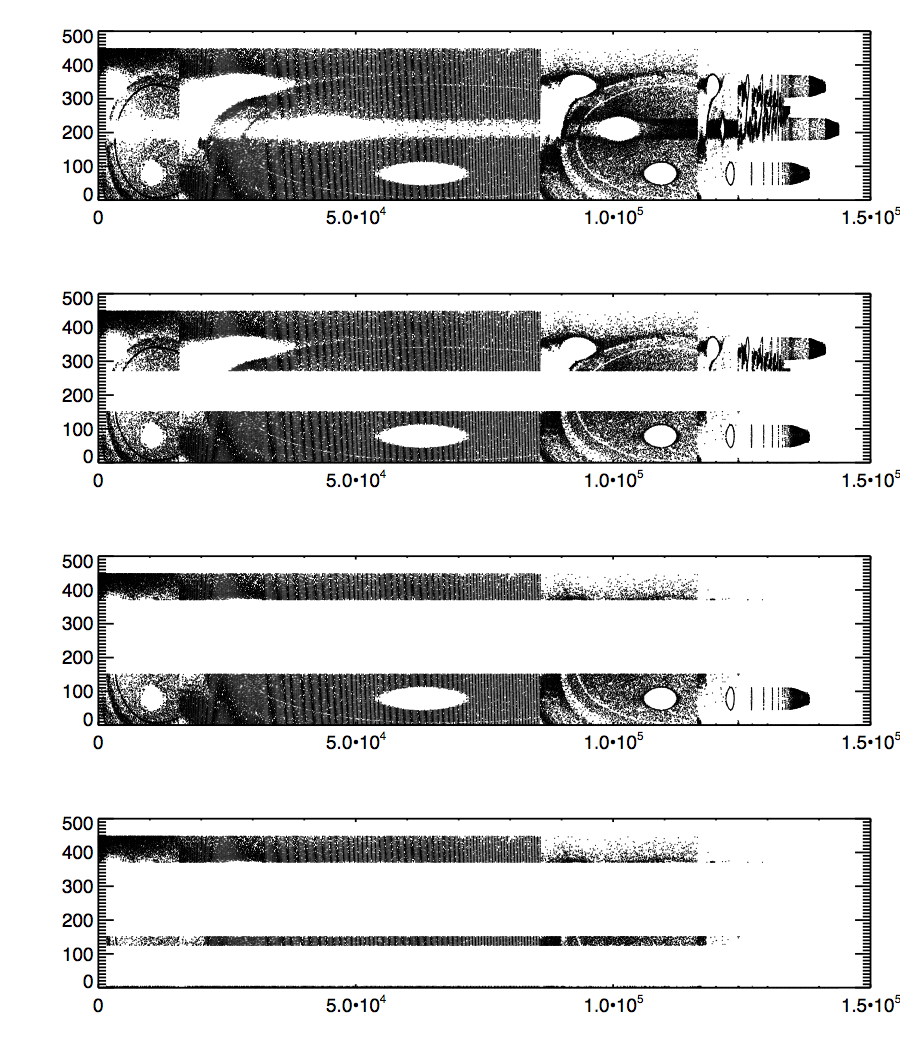
\includegraphics[width=\textwidth]{../plots_tables_images/quickcenters.eps}%
   \caption{The 2D array sorted by x or y positions}\label{sortsort}
\end{figure}

From the approximate centers, we crop a box around the sun and slice rows/columns of data. Next, we limb fit the edges of the sun so that we can find more accurate center positions. At first we used a 3 order fit, then a linear fit (since that's what Albert used), then to a 2nd order fit (because we thought it wasn't good enough) then back to a linear fit (because the fit was good enough). 

\subsection{Thresholds} % (fold)
\label{sub:thresholds}
We want a robust threshold so instead of using an arbitrary parameter multiplied by the max of the image, we sort the 2D image into a 1D array and return the position of the boundaries of the regions which are seen as humps.

To find the boundaries, we look at the 2nd derivative of the sorted array and find the 3 maximum peaks (in the case of 3 suns), corresponding to the boundaries of the aforementioned humps. We chose this way because thresholding the peaks requires parameterization that needs to be changed dynamically. 

\begin{figure}[!ht]
   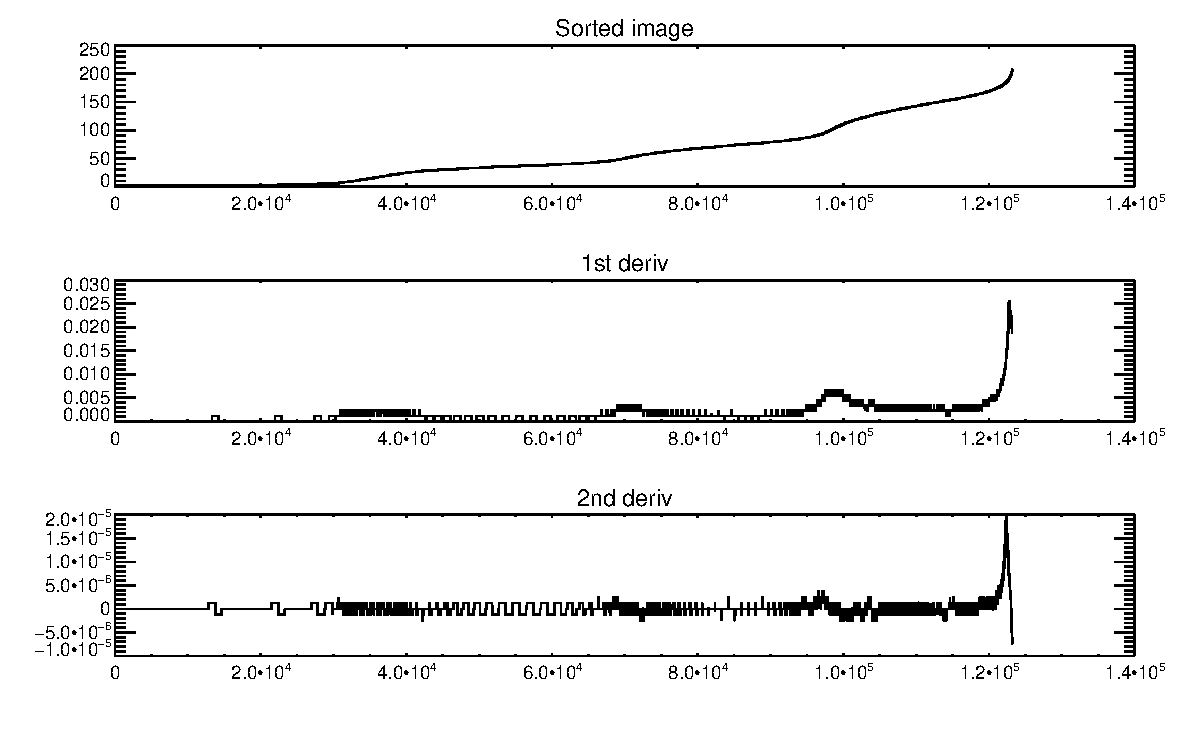
\includegraphics[width=.75\textwidth]{../plots_tables_images/sortedarray.eps}%
   \caption{This is the sorted array for a 3-sun image. The peaks don't look that large in the second derivative, but that's just because of the scaling to the first peak.}\label{peaks}
\end{figure}

Several factors affecting thresholding values:

\begin{enumerate}
    \item \hl{\texttt{smooth()}} parameters
    \item Unusually bright pixels
    \item artifacts of smoothing
\end{enumerate}

To solve 1), we used the \hl{\texttt{edge\_truncate}} keyword because it gave us the least amount of weird edge artifacts in the 1D array. The other options were \hl{\texttt{edge\_zero}} and \hl{\texttt{edge\_mirror}} which yielded poor results.

To solve 2), when we sorted the array by brightness, we left out the top .1\% of the pixels.

To solve 3), we had to manually cut off the last 10,000 pixels. This part needs to be improved.

% subsection thresholds (end)
% section finding_centers_of_sun (end)

\section{Finding Fiducial Positions} % (fold)
\label{sec:finding_fiducial_positions}

Now that we have a limb-fitted centroid, we analyze the sun for fiducials. They are characteristically dark, so we ended up looking at 1D sums in the row/column directions and looking for wide dips in brightness (where 1D sum lines up with the entire length of the fiducial). Before this method, we looked at a few other options. They included:

\begin{enumerate}
    \item Running edge detector filters to isolate the edge of the fiducials
    \item Applying convolution/cross-correlation filters 
\end{enumerate}

For edge detection filters, we looked at \hl{\texttt{emboss}}, \hl{\texttt{shift\_diff}}, and \hl{\texttt{laplacian}}. Using 2D filters posed a few problems. One, it was time consuming because it required processing on a 2D array. Two, the result was a 2D array that we had to further process. The basics of the edge detection filters was that when run with a kernel that emphasized an edge of the fiducial, we get an array that traces out the shape of the fiducial (to some extent). For the case of \hl{\texttt{shift\_diff}}, a high value corresponds to a leading edge and a low value to a falling edge. We threshold the 2D image for a high threshold so we retrieve all the leading edges in a certain direction. Next, we see where in the image the leading edges are so that we can pinpoint exact fiducial positions. 

\begin{figure}[!ht]
   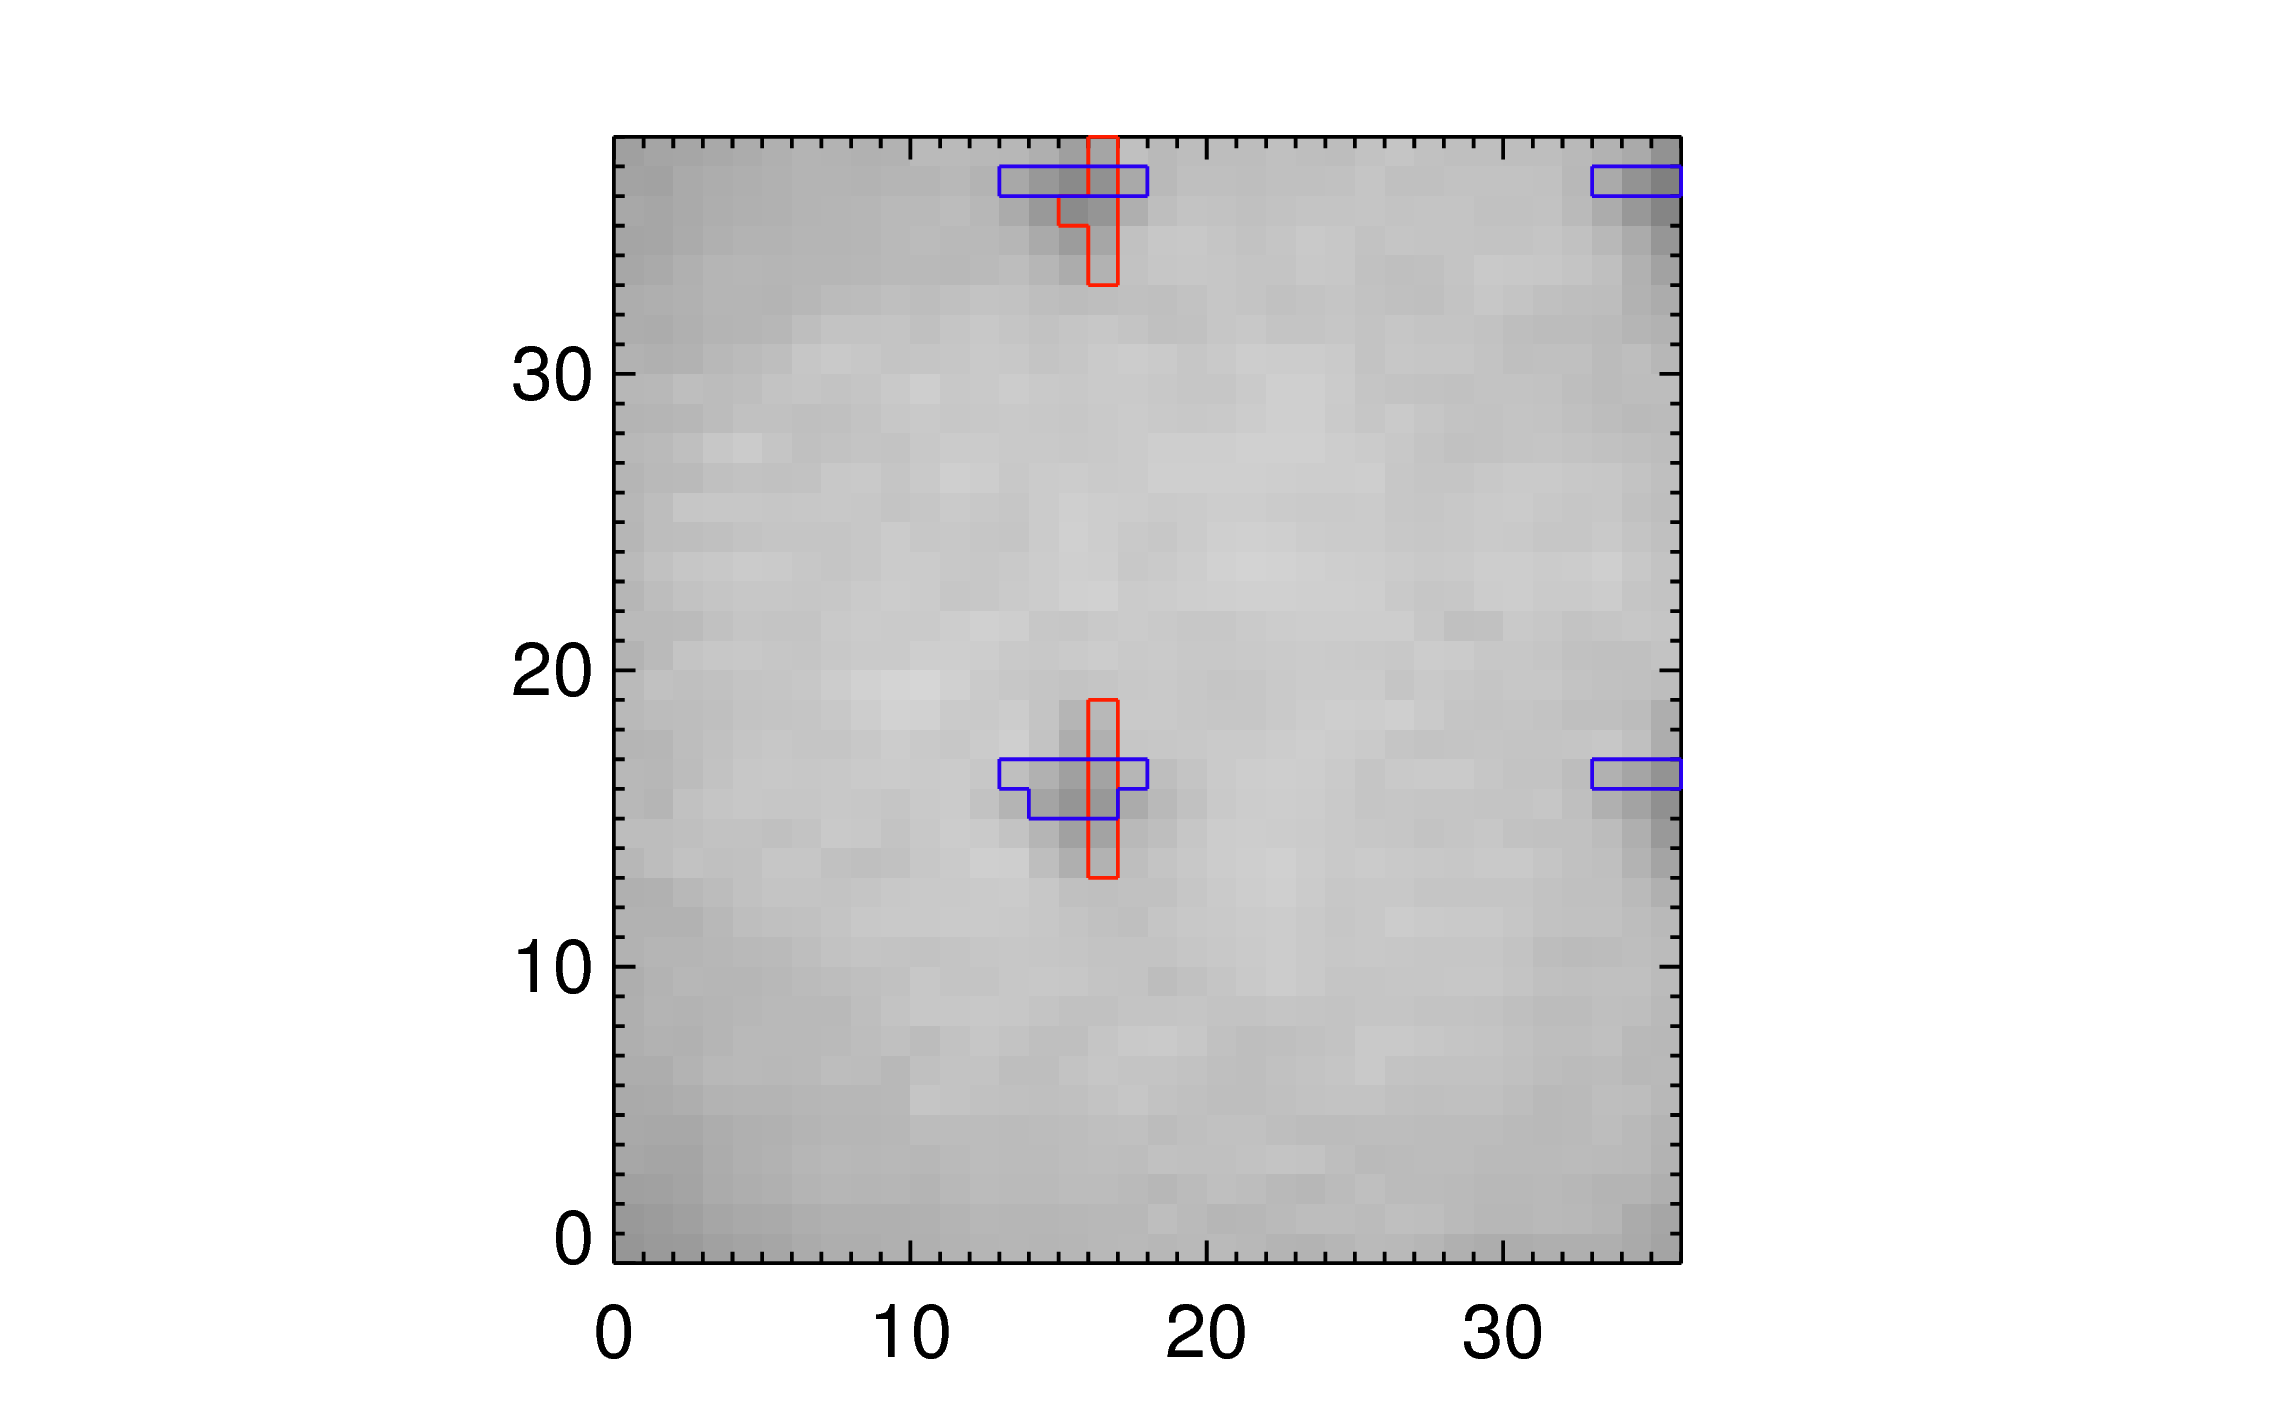
\includegraphics[width=.75\textwidth]{../plots_tables_images/threshtesh_3.png}%
   \caption{The pixels outlined correspond to values from the edge detection-filtered array}\label{edge_det}
\end{figure}

One issue was that the method used involved returning only the x and y positions of each fiducial candidate in no specific order. They weren't paired up in a certain way so we got a long list of $x$ and $y$ positions. We had to look at each possible fiducial pair and determine if there was actually a fiducial there or not (is the pixel value at the coordinate dim enough). Then, we checked to see if the fiducial coordinate was more than a certain distance from the solar center (because we only care about fiducials close to the center anyhow). Once it passed this second check, we cropped a small area around the fiducial candidate and looked at the 1D sums per row/column. If there is a dip (characteristic of a fiducial), then the fiducial candidate is confirmed as an actual fiducial.\\

In addition to using edge detection filters to find fiducials, we also looked at a convolution/cross correlation filter. I mention cross correlation because it is the method Albert used in his image analysis code. Convolution and edge detection filters only differ by the shape and content of the kernel so it required many a tweaks to find one that emphasized the shape of the fiducial while suppressing foreign noise and shapes. What we ended up with was 

\begin{figure}[!ht]
   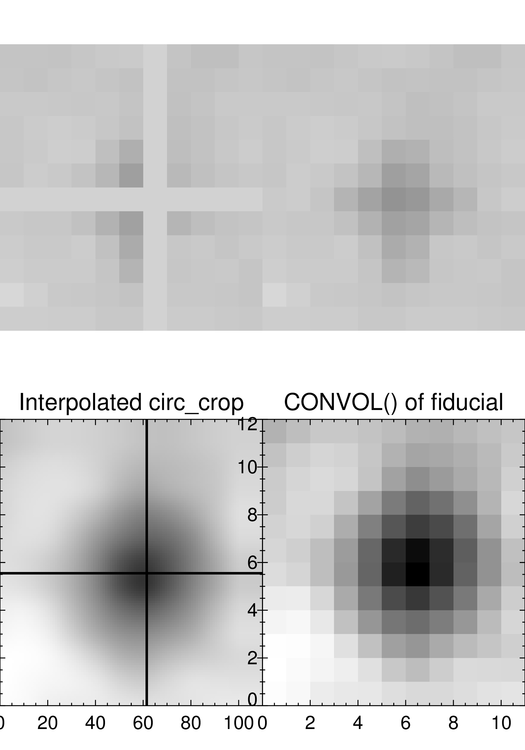
\includegraphics[width=.75\textwidth]{../plots_tables_images/cropcomp3.png}%
   \caption{w}\label{cropcomp}
\end{figure}

Another problem related to fiducial finding is dealing with fiducials on the edge of the sun. If a fiducial lies on the edge, it is hard to distinguish from the edge pixels without some sort of spatial information, like a convolution filter. Currently we don't have a method to deal with dim fiducials on the edge because we only care about the 4 brightest fiducials to the center of the sun. 

% section finding_fiducial_positions (end)

\section{Miscellaneous} % (fold)
\label{sec:miscellaneous}
Extra
% section miscellaneous (end)


\end{document}

he picked you up
nice shirt
so laugh
so cool
omg fun
such hug
hold me plz









